\documentclass{beamer}
\usepackage{geometry}
\usepackage[english]{babel}
\usepackage[utf8]{inputenc}
\usepackage{amsmath}
\usepackage{amsfonts}
\usepackage{amssymb}
\usepackage{tikz}
\usetikzlibrary{quotes, angles}
\usepackage{graphicx}
\usepackage{multicol}

%\usepackage{pgfplots}
%\pgfplotsset{width=10cm,compat=1.9}
%\usepackage{pgfplotstable}

\setlength{\headheight}{26pt}%doesn't seem to fix warning

\usepackage{fancyhdr}
\pagestyle{fancy}
\fancyhf{}

%\rhead{\small{3 September 2019}}
\lhead{\small{BECA / Dr. Huson / Geometry Unit 1}}

\renewcommand{\headrulewidth}{0pt}

\title{Mathematics Class Slides}
\subtitle{Bronx Early College Academy}
\author{Christopher J. Huson PhD}
\date{7-15 October 2020}

\begin{document}
\frame{\titlepage}
\section[Outline]{}
\frame{\tableofcontents}

\section{1.10 Assessment results, 14 October}
  \frame
  {
    \frametitle{GQ: How do we measure our efforts and results?}
    \framesubtitle{CCSS: HSG.CO.A.1 Know precise geometric definitions  \hfill \alert{1.10 Wednesday 14 Oct}}
  
    \begin{block}{Do Now: Self-assessments questions}
    \begin{enumerate}
        \item How do we work efficiently and become a good scholar
        \item What should we know and be able to do
    \end{enumerate}
    \end{block}
    Lesson: Circle definition, trisection \\
    Review and practice of vocabulary, line segments, and congruence
  }

  \frame
  {
    \frametitle{Scholarship assessment}
    \framesubtitle{1: Well below, 2: Approaching, 3: Meets expectations, 4: Exceeds}
  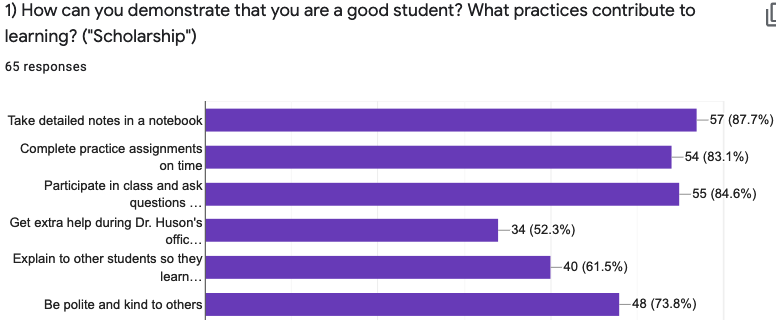
\includegraphics[width=.95\textwidth]{scholarship-bar-chart.png}
    \begin{enumerate}
      \item Participate: Attendance (Google Classroom), Classkick
      \item Practice assignments: Khan Academy, Deltamath, 1.5 worksheet
      \item Detailed notes: Notebook treasure hunt uploads (weekend)
    \end{enumerate}
  }

  \frame
  {
    \frametitle{What do I know, what can I do assessment}
    \framesubtitle{1: Well below, 2: Approaching, 3: Meets expectations, 4: Exceeds}
  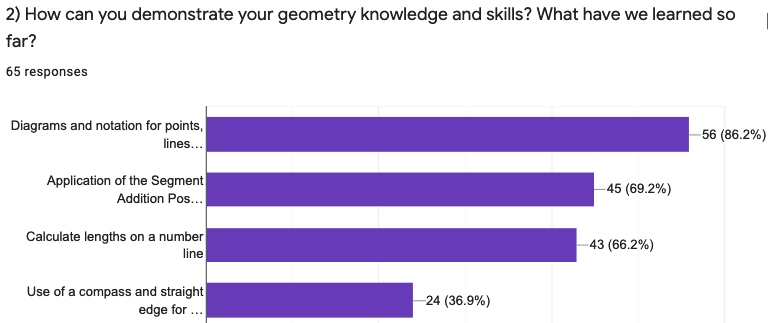
\includegraphics[width=.95\textwidth]{know+do-bar-chart.png}
    \begin{enumerate}
      \item Classkick (open book, timed; use @beca324.org login):\\ Diagrams \& notation, segment addition, number line lengths
      \item Project: Construction of an equilateral triangle
    \end{enumerate}
  }

  \frame
  {
    \frametitle{Scholarship: Participation in synchronous classes}
      Participation with classmates in the lessons conducted by the teacher is one of the primary inputs to learning.\\[0.25cm]
      Among Geometry students, $84.6\%$ considered it important. \vspace{0.5cm}
      \begin{table}[ht]
        \textbf{Participation Grade}
      \begin{tabular}[t]{p{0.25\linewidth} c c c }%{|p{2.4cm}|p{5.5cm}|p{8cm}|p{4cm}|}
        \hline
        1. Well below \newline expectations & 2. Approaching & 3. Meets & 4. Exceeds \\
        \hline
        \hspace{0.5cm}$<75\%$ & 75+\% & 100\% &  \\[0.25cm]
        \multicolumn{4}{c}{based on 11 assignments in Google Classroom (no late penalty)} \\[0.25cm]
        \hline
      \end{tabular}
    \end{table} \vspace{0.25cm}
      You must also load Genuis Scan and register in \emph{Classkick} as a portfolio user, or lose one level
      \vspace{1cm}
  }

  \frame
  {
    \frametitle{Scholarship: Practice assignments}
      ``Doing your work'' is how math skills and knowledge are gained.\\[0.25cm]
      Completing assignments on time was cited by $83.1\%$ of students. \vspace{0.5cm}
      \begin{table}[ht]
        \textbf{Practice Grade}
      \begin{tabular}[t]{p{0.25\linewidth} c c c }%{|p{2.4cm}|p{5.5cm}|p{8cm}|p{4cm}|}
        \hline
        1. Well below \newline expectations & 2. Approaching & 3. Meets & 4. Exceeds \\
        \hline
        \hspace{0.25cm} 0 or 1 out of 5 & 2 / 5 & 3 or 4 / 5 & 5/5 \\[0.25cm]
        \multicolumn{4}{c}{1.1 Khan Academy, Deltamath (3), 1.5 Worksheet} \\[0.25cm]
        \hline
      \end{tabular}
    \end{table} \vspace{0.25cm}
      Satisfactory completion of an assignment requires \emph{effort}, but not perfection. (a score of $65\%$ is usually sufficient)
      \vspace{1cm}
  }

  \frame
  {
    \frametitle{Scholarship: Taking notes}
      Writing mathematics helps you learn and gives you notes to study.\\[0.25cm]
      Students said taking notes in a notebook was the most important practice for successful learning $87.7\%$. \vspace{0.5cm}
      \begin{table}[ht]
        \textbf{Notebook Grade}
      \begin{tabular}[t]{p{0.25\linewidth} p{0.25\linewidth} p{0.15\linewidth} p{0.25\linewidth}}
        \hline
        1. Well below \newline expectations & 2. Approaching & 3. Meets & 4. Exceeds \\
        \hline
        Missing several notes & Largely complete & Detailed, \newline complete & Detailed, complete, neat \& organized \\[0.25cm]
        \multicolumn{4}{c}{1.10 Notebook ``treasure hunt''} \\[0.25cm]
        \hline
      \end{tabular}
    \end{table} \vspace{0.25cm}
      Scan of pages must be uploaded (Genius app) \\one level penalty otherwise
      \vspace{1cm}
  }
  
  \end{document}